%
% $RCSfile: observer.tex,v $
%
% Copyright (c) 2004. Christian Heller. All rights reserved.
%
% No copying, altering, distribution or any other actions concerning this
% document, except after explicit permission by the author!
% At some later point in time, this document is planned to be put under
% the GNU FDL license. For now, _everything_ is _restricted_ by the author.
%
% http://www.cybop.net
% - Cybernetics Oriented Programming -
%
% http://www.resmedicinae.org
% - Information in Medicine -
%
% @author Christian Heller <christian.heller@tuxtax.de>
%

\paragraph{Observer}
\label{observer_heading}

Another pattern that found wide application is the \emph{Observer} \cite{gamma1995},
an often-used synonym for which is \emph{Publisher-Subscriber}. It provides a
notification mechanism for all objects that registered as \emph{Observer} at a
\emph{Subject} in whose state changes they are interested, leading to an automatic
update of all dependent objects (figure \ref{observer_figure}).

\begin{figure}[ht]
    \begin{center}
        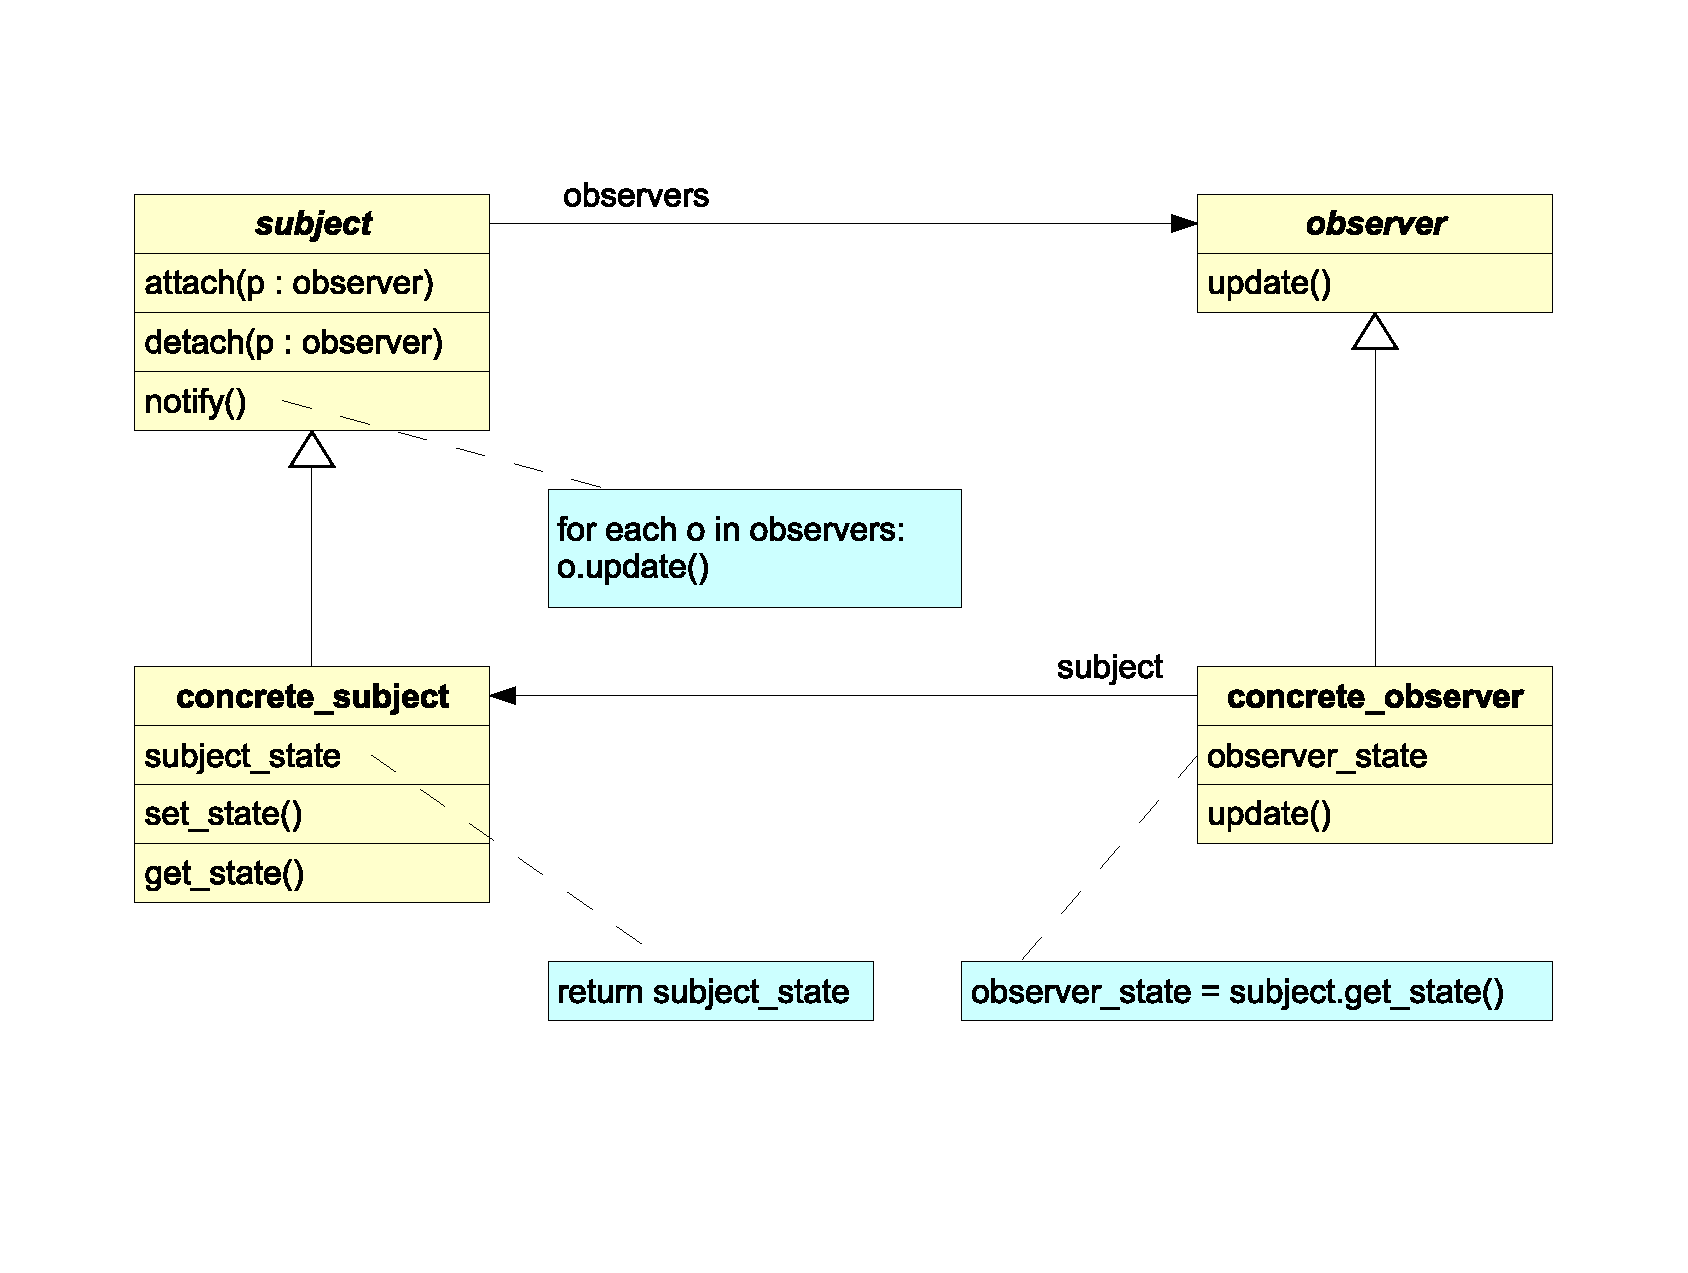
\includegraphics[scale=0.3]{vector/observer.eps}
        \caption{Observer Pattern}
        \label{observer_figure}
    \end{center}
\end{figure}

\begin{figure}[ht]
    \begin{center}
        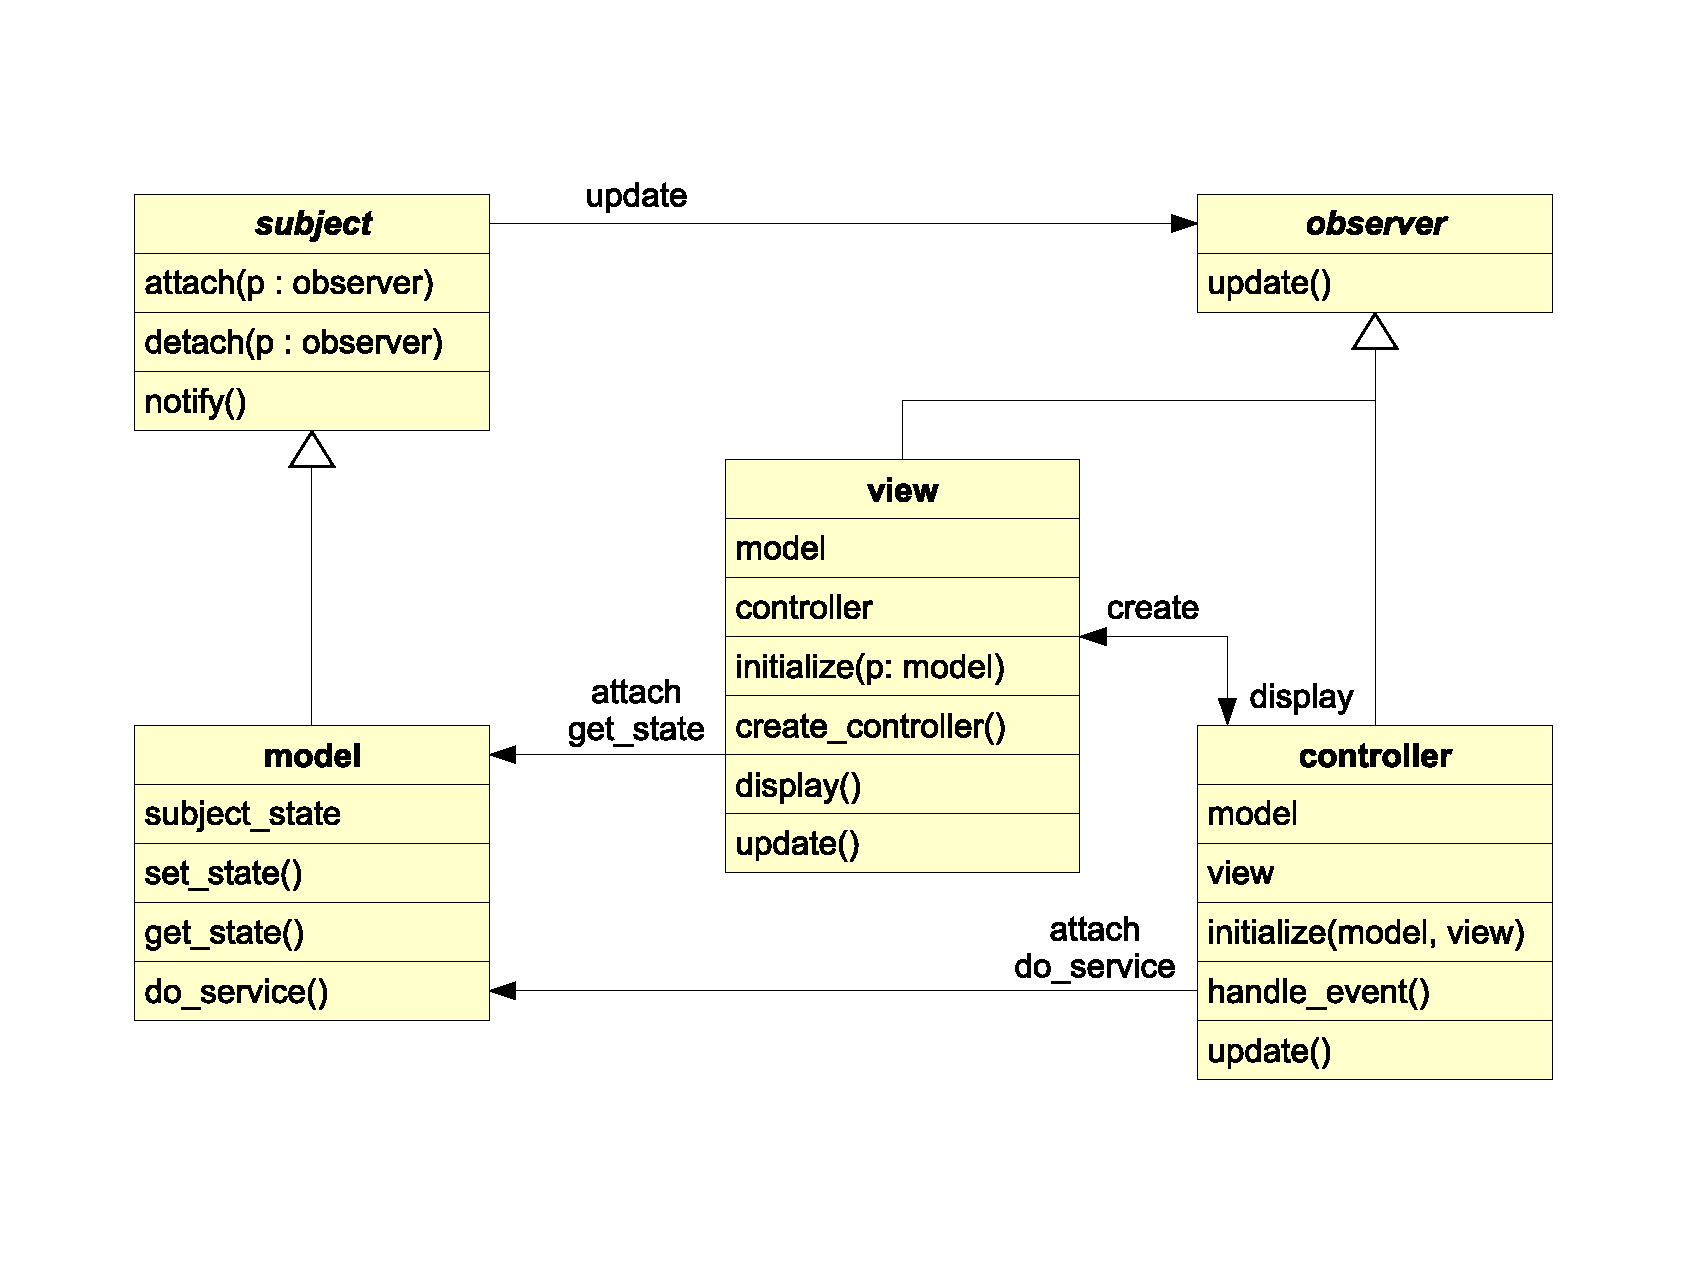
\includegraphics[scale=0.3]{vector/mvcobserver.eps}
        \caption{MVC- using Observer Pattern}
        \label{mvcobserver_figure}
    \end{center}
\end{figure}

Similar notification mechanisms are used for \emph{Callback} event handling in
frameworks, where the framework core calls functionality of its extensions. The
\emph{Model View Controller-} (MVC) uses the \emph{Observer} pattern to let the
model notify its observing views about necessary updates (figure
\ref{mvcobserver_figure}).

A disadvantage of the \emph{Observer} pattern is that it relies on bidirectional
dependencies (section \ref{bidirectional_dependency_heading}), so that circular
references can occur, when a system is not programmed very carefully.
